\chapter{Theoretical Framework}
\label{chap:background}

This chapter presents the theoretical foundations and state of the art related to \gls{mcp} and its security implications. It reviews \gls{mcp} architectures, adversarial risks, and existing research on securing tool-augmented and multi-agent \gls{ai} systems. Relevant methodologies and related studies are also discussed to establish the conceptual basis for the proposed tool.   

\section{Large Language Models and Agentic AI}
% TODO (this turn deferred by scope): expand this section.
% Cover: what an LLM is at the level this thesis needs (next-token prediction,
% instruction following, context window as the single trust-blind channel);
% the shift from a model that only emits text to an agent that calls tools and
% acts; why the inability to separate instructions from data in the context
% window is the root cause that the rest of the chapter builds on. Keep it short
% and in service of the security argument, not an LLM tutorial.
Large language models predict text from a context window that mixes system instructions, user input, and any external content retrieved at runtime. The model does not maintain a reliable boundary between these sources: an instruction embedded in retrieved data is read with the same weight as an instruction from the system prompt. When such a model is given the ability to invoke tools, it becomes an agent whose actions in the world are driven by that same undifferentiated context. This property is the root cause from which the attack surface discussed in the remainder of this chapter follows, and it is why defenses that assume a clean separation between trusted and untrusted input do not transfer directly to \gls{llm}-driven systems.

\section{Model Context Protocol and Agentic AI Architectures}

The \gls{mcp} enables large language models (\gls{llm}s) to interact with external tools, databases, and services through structured communication mechanisms \citep{anthropic2024mcp}. Unlike traditional \gls{ml} systems that operate within static inference environments, \gls{mcp}-based systems function as distributed, tool-augmented \gls{ai} architectures \citep{mitre2023atlas} in which language models may initiate external actions, retrieve contextual information, and collaborate with other agents.

From a systems perspective, \gls{mcp} introduces multiple execution layers and trust boundaries, as shown in Figure~\ref{fig:2}:

\newpage

\begin{figure}[htb]
    \centering
    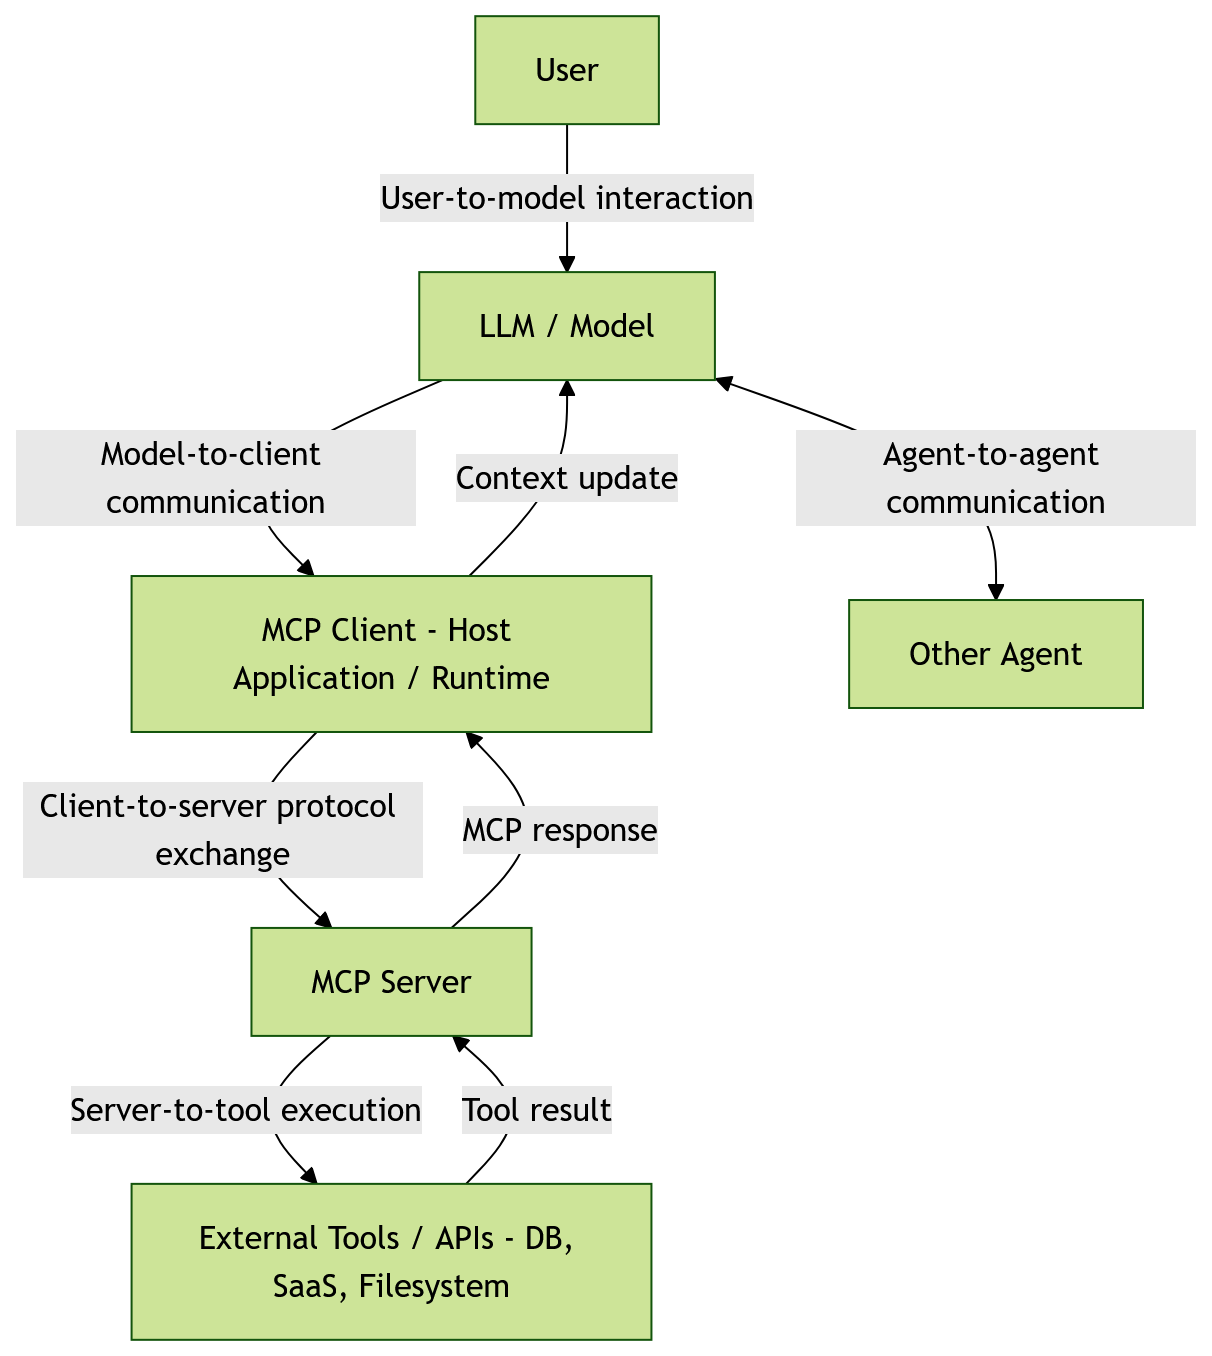
\includegraphics[width=0.8\linewidth]{images/mermaid-diagram-2026-02-23-233324.png}
    \caption{MCP Interactions Diagram}
    \label{fig:2}
\end{figure}

Each boundary represents a potential attack surface. In distributed systems theory, security risk increases with the number of interfaces and execution paths exposed to external input \citep{manadhata2011attack}. \gls{mcp} formalizes these interfaces and therefore structurally expands the attack surface of \gls{ai}-driven systems. This architectural shift necessitates security models that account for both protocol-level manipulation and semantic manipulation of model behavior.

\section{Attack Surface Expansion in Tool-Augmented LLM Systems}

Attack surface theory posits that the security exposure of a system grows as new interfaces, communication channels, and privilege domains are introduced \citep{manadhata2011attack, nist2022ssdf}. 
In \gls{mcp}-enabled environments, the attack surface expands along three principal dimensions:

\begin{enumerate}
    \item \textbf{External tool invocation} – \gls{llm}s are capable of triggering external tools based on natural language instructions. This introduces risks related to improper input validation, command injection, and unintended execution of sensitive operations. If tool interfaces are not strictly constrained, malicious or manipulated prompts may lead to unauthorized actions being performed at the system level.
 

    \item \textbf{Permission and authorization management} – MCP architectures rely on permission boundaries to control which tools and resources an agent can access. Weak or misconfigured access control mechanisms may allow privilege escalation, enabling agents to perform actions beyond their intended scope. Ensuring strict enforcement of least-privilege principles is therefore critical.

    \item \textbf{Multi-agent communication flows} – In systems involving \gls{a2a} communication, agents exchange information and delegate tasks. This introduces risks such as trust boundary violations, propagation of malicious instructions across agents, and cascading compromise scenarios where a single compromised agent affects the entire system.
\end{enumerate}

Unlike traditional web applications, \gls{mcp} systems combine probabilistic reasoning (\gls{llm} inference) with deterministic execution (tool invocation). This hybrid execution model creates a class of vulnerabilities in which semantic manipulation through natural language may result in concrete system-level actions \citep{greshake2023prompt, mitre2023atlas}. Therefore, \gls{mcp} security must be analyzed not only through classical input validation models but also through adversarial reasoning tools. Some \gls{mcp} systems may also involve contextual data retrieval mechanisms, which can introduce additional security considerations; however, this aspect is outside the scope of this work.

\section{Adversarial Machine Learning and Prompt Injection}

Adversarial \gls{ml} provides the theoretical foundation for understanding how \gls{ai} systems can be manipulated through crafted inputs. In \gls{llm}-based architectures, adversarial behavior most commonly manifests as \gls{prompt_injection}.

Prompt injection exploits the model’s reliance on contextual instructions \citep{greshake2023prompt, liu2024universal}, attempting to override system-level constraints or introduce malicious operational directives. In \gls{mcp} environments, such attacks may induce:

\begin{itemize}
    \item Unauthorized tool execution,
    \item Privilege escalation,
    \item Data exfiltration,
    \item Cross-agent contamination.
\end{itemize}

These attack vectors are particularly challenging to mitigate due to the probabilistic nature of \gls{llm} behavior. Unlike traditional software systems, where execution paths are explicitly defined, \gls{llm}s interpret instructions based on contextual understanding, making it difficult to enforce strict separation between trusted and untrusted inputs \citep{greshake2023prompt, liu2024universal}.

Furthermore, prompt injection can be indirect, where malicious instructions are embedded in external data sources such as web pages, documents, or database entries retrieved at runtime. This significantly broadens the threat landscape, as attackers do not need direct access to the system prompt to influence model behavior.

As a result, effective mitigation requires a combination of techniques, including input sanitization, contextual isolation, permission-aware execution, and continuous adversarial testing. These approaches shift security from purely preventive mechanisms to adaptive and resilience-based strategies.

Theoretical work on adversarial robustness demonstrates that language models cannot reliably distinguish between benign and malicious instructions embedded within contextual data. Consequently, defense strategies must rely on architectural safeguards, permission enforcement, validation layers, and adversarial testing rather than purely on model alignment techniques.

\section{Threat Modeling in Protocol-Driven AI Systems}

\gls{threat_modeling} is a structured methodology for identifying and categorizing vulnerabilities across system components and trust boundaries. In distributed and protocol-driven systems, methodologies such as STRIDE (Spoofing, Tampering, Repudiation, Information Disclosure, Denial of Service, Elevation of Privilege) provide systematic coverage of security risks \citep{mitre2023atlas}.

This implies that threat modeling must consider not only classical vulnerabilities but also how contextual inputs can influence system behavior. For example, a seemingly benign prompt may lead to unintended tool execution if the model misinterprets intent or if safeguards are insufficient.


Applying threat modeling to \gls{mcp} involves analyzing:

\begin{itemize}
    \item Authentication and identity validation between client and server,
    \item Integrity of contextual payloads,
    \item Confidentiality of retrieved resources,
    \item Authorization boundaries governing tool execution,
    \item Lateral movement across agents in \gls{a2a} scenarios.
\end{itemize}

Formal threat modeling enables classification of vulnerabilities and supports the design of automated detection mechanisms. This theoretical foundation directly informs the development of the \gls{mcp} security scanning agent proposed in this research.

\section{Automated Vulnerability Detection and Continuous Validation}

Modern cybersecurity practice relies on automated vulnerability detection mechanisms, combining static analysis, dynamic testing, and adversarial simulation \citep{owasp2025thirdparty, owasp2024llm01}.

\gls{static_analysis} enables detection of structural weaknesses in source code, such as improper permission handling or insecure token validation. \gls{dynamic_testing} evaluates runtime behavior under controlled adversarial conditions.

In addition to traditional techniques, MCP security requires \textbf{semantic adversarial testing}, where malicious or crafted prompts are systematically generated to evaluate how \gls{llm}-driven systems respond to adversarial inputs. This form of testing targets vulnerabilities that arise from the interpretation of natural language, including \gls{prompt_injection}, context manipulation, and unintended action triggering \citep{greshake2023prompt, liu2024universal}.


Continuous validation aligns with \gls{defense_in_depth} theory \citep{nist2022ssdf}, which advocates layered security mechanisms rather than reliance on a single control. Integrating automated security scanning into development pipelines allows \gls{mcp} implementations to be re-evaluated not only at design time but also later in their lifecycle.


Together, these foundations justify the development of a secure development and testing tool for \gls{mcp} implementations and provide the conceptual basis for the automated \gls{mcp} security scanning agent proposed in this dissertation.